% Chapter 1

\chapter{Introduction} % Main chapter title

\label{Chapter1} % For referencing the chapter elsewhere, use \ref{Chapter1} 

\lhead{Chapter 1. \emph{Introduction}} % This is for the header on each page - perhaps a shortened title

%----------------------------------------------------------------------------------------
%\DeclareMathOperator*{\Min}{Min}
The most important goal in this thesis is to find a solution of the nonsmooth minimization problem

\begin{equation} \label{mainproblem}
  \begin{aligned}
    & \underset{x \in \mathbb{R}^n}{\text{min}}
    & & f(x) \\
    & \text{s.t.}
    & & l_i \leq x_i \leq u_i , \; \\
    & & & i = 1, \ldots, n.
  \end{aligned}
\end{equation}

where $f \colon \mathbb{R}^n \to \mathbb{R}$.  And $l_i$ and $u_i \in \mathbb{R}$

In the particular case when $n = 0$, the problem would be called "unconstrained" and while it is still an open subject that needs to be better understood.  Several techniques have already been developed to handle this type of problems \citep{unconstrained}.  In our particular case $n$ is supposed to be finite but very large. A larger problem not only means that the problem will take a longer time to solve compared to a similar problem. But storing and calculating a Hessian matrix is prohibitively expensive.  In this thesis $f(x)$ is a nonsmooth continuous function, that is, the function $f(x)$ itself is continuous but its gradient $\nabla f(x)$ is not.

For the particular case when $n$ is a small number, several methods that solve optimization problems of nondifferentiable functions in lower dimensions \citep{kiwiel85} have been developed.  In the case of smooth functions, it is possible to use Newton iteration algorithms and achieve quadratic convergence, the problem with Newton algorithms is that they require second derivatives to be provided\footnote{the main issue with the second derivative is that it requires a total of $n \times n$ partial derivatives.  Which is impractical for medium and for some small-size problems}.  In the 1950's and several years after that, several quasi-newton methods were proposed where the second derivative Hessian matrix is "approximated" step by step \citep{unconstrained}.  These approximations or "updates" are calculated after every iteration and the way in which this update is found defines a new method depending on the particular needs.  This thesis will only be concerned with the $BFGS$.  \footnote{BFGS stands for the last names of its authors Broyden, Fletcher, Goldfarb and Shanno} which can achieve super linear convergence, has proven to work in most practical purposes and posseses very nice self correcting features \citep{selfcorrecting}, in other words, it doesn't matter that one update incorrectly estimates the curvature in the objective function,  It will always correct itself in just a few steps.  This self-correcting property is very desired in the nonsmooth case, since changes in curvature could be large near the optimal point.   $BFGS$ is not the only update method available, there are many more updates typically used.  In particular we have the SR1(Symmetric Rank-1), which has the problem that it may not maintain a positive definiteness of the Hessian in the case when f is convex, although it otherwise generates "good Hessian approximations"\citep{nocedal} Another update worth mentioning is the $DFP$\footnote{DFP also stands for its authors Davidon, Fletcher and Powell.  Davidon is credited with the first quasi-newton algorithm.  He developed it while he was working at Argonne National Laboratories} which together with BFGS spans the Broyden class of updates.

Finally, this thesis will also assume that the Hessian matrix is not sparse.  In this case, there are other algorithms that may be more suitable \citep{Fletcher96computingsparse, sparse}, some of them have even been implemented in fortran \citep{lancelot}.

In this sense, chapter \ref{ChapterBFGS} will extend on $BFGS$ and on the basic reasons and steps to move into a large scale $L-BFGS$.  During the solution of an unconstrained problem, a template version of $C++$ code was created which enhances the code originally written by Allan Kaku and Anders Skaaja \citep{kaku}.  This software maintains Allan's high-precision libraries.  A link to this $BFGS+L-BFGS$ software is provided in the thesis website.  An introduction to the different quasi-newton methods is provided, with a simple introduction to the most important of them and the some of the most basic techniques to guarantee a reasonable speed of convergence.

The next chapter is chapter \ref{ChapterConstraints} and this chapter introduces the algorithm by Nocedal, and what changes were introduced into the code in order to produce a better and stable version in the nonsmooth case.  The website also contains a $FORTRAN$ implementation derived from the original implementation by Nocedal.

Nocedal's original algorithm consists of $2$ steps.  In the first step most of the dimensions in the problem should be removed, making the problem a lot simpler.  And in the second step there is some fine tuning to guarantee better than just linear speed of convergence.

\chapter{BFGS and L-BFGS and implementations in the unconstrained case}
\label{ChapterBFGS} % For referencing the chapter elsewhere, use \ref{ChapterBFGS}

The $BFGS$ method is a line search method. For this reason an introduction to line search methods is important

\section{Line Search Methods:}

Line search methods are iterative methods where every step the researcher has to decide a direction to move or "search direction" and also, how much to move in that direction or "step length".  In general all line search methods are characterized by the equation

\begin{equation} \label{basiclinesearch}
  x_{k+1} = x_k + \alpha_k d_k
\end{equation}

where $\alpha_k$ is the step length and $d_k$ is the search direction.

The main difference between line search methods will be in the selection of $\alpha_k$ and $d_k$ and depending on this selection it will be possible to achieve a convergence that will typically be somewhere between linear and quadratic.

In general it is desirable that the search direction is a descent direction in every step.  So one usually also checks that the property $d_k^T \nabla f_k = |d_k||\nabla f_k| \cos{\theta} < 0$ is satisfied.

In general the search direction will have the form 

\begin{equation} \label{searchdirection}
    \begin{aligned}
      d_k = -B_{k}^{-1} \nabla f_k
    \end{aligned}
\end{equation}
 
And the choice of matrix $B_k$ will define what type of method we are using.  This implies that together with the search direction condition with  $d_k^T \nabla f_k < 0$ we need that:

\begin{equation} \label{Bposdef}
  \begin{aligned}
    -\nabla f_k B_k^{-1} \nabla f_k < 0
  \end{aligned}
\end{equation}

And this would require that $B_k$ be positive definite.

Other conditions that are of the utmost importance in this thesis are the conditions on step length.  These conditions are so important in this thesis that they will be reviewed in a separate chapter.  
 
Next a presentation of some  of the most important line search methods

\subsection{Steepest Descent}

The most naive choice of search direction is the negative of the gradient $\nabla f_k(x)$, which is equivalent to choosing $B_k = I$.  This method is called steepest descent and its main advantage is obviously that it only requires $\nabla f_k$ as an input.

If the condition of the function's Hessian matrix is low, then steepest descent will converge very fast,  but if this condition is high, the method will take a lot of iterations.  In the worst cases, steepest descent can show a zig-zagging pattern that slows down convergence.

\begin{figure}[htbp]
  \centering
  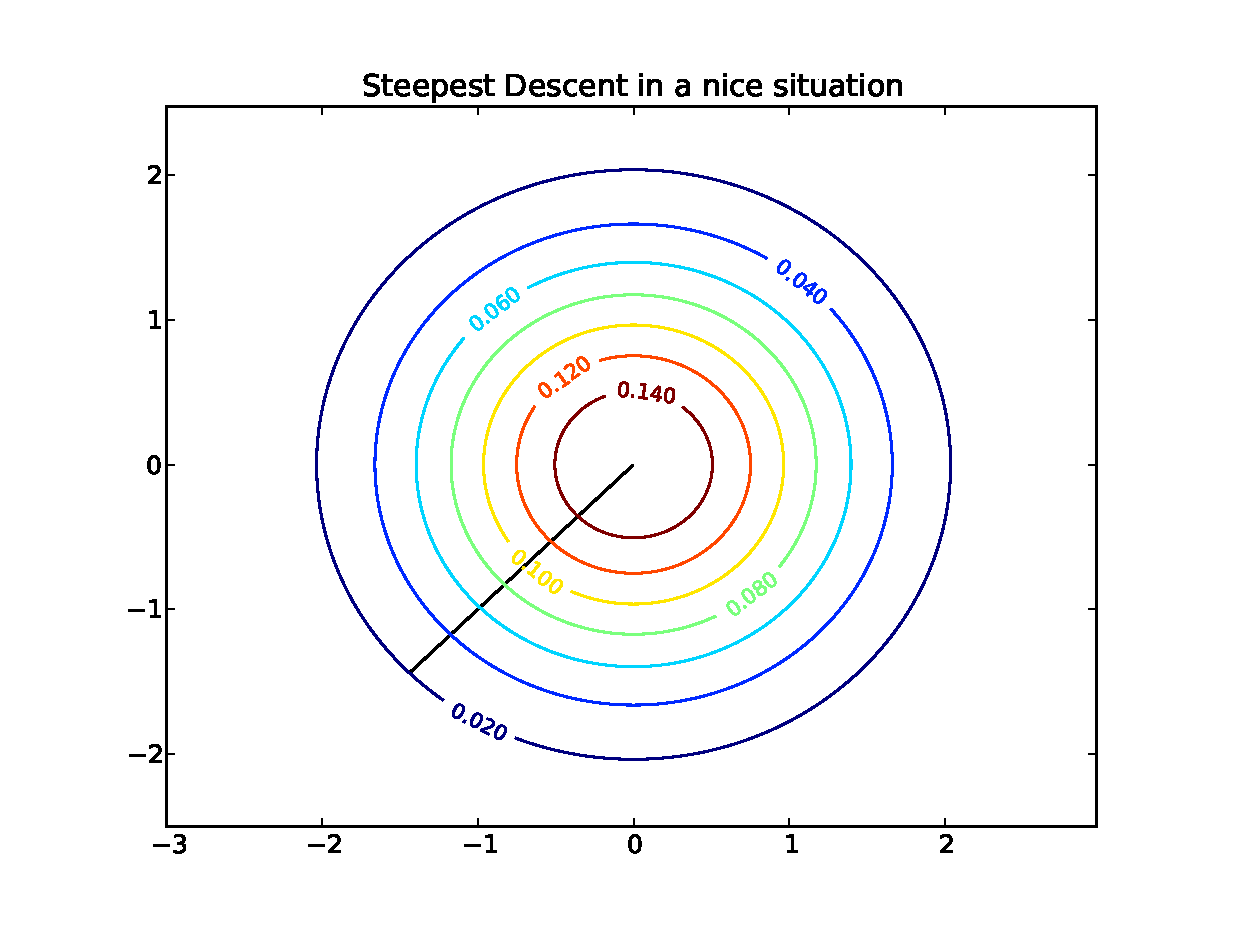
\includegraphics[width=2.5cm]{Figures/steepestDescentNice}
  \rule{35em}{0.1pt}
  \caption[step. Desc.]{Steepest Descent exampel}
  \label{fig:steepestdescent}
\end{figure}

\subsection{Newton's Method}

Newton's method highly improves upon steepest descent by incorporating information from the Hessian second derivative.   It's derivation comes from the second-order Taylor series model of the function around the current point $x_k$. 

\begin{equation} \label{secondorderTaylor}
  \begin{aligned}
    f(x_k + d_k) = f(x_k) + d_k^T \nabla f_k + \frac{d_k^T \nabla ^2 f_k d_k}{2}  
  \end{aligned}
\end{equation}

And assuming positive definitiness of the Hessian matrix, the optimal value of $d_k$ can be obtained by deriving and equating to zero.  Thus the direction is determined by the following formula.

\begin{equation} \label{NewtonDir}
  \begin{aligned}
    d_k^N = -\left(\nabla^2 f(x_k) \right)^{-1} \nabla f(x_k)
  \end{aligned}
\end{equation}

This new search direction stablishes a change in the metric by means of the Hessian matrix $\nabla ^2 f$.  With this change, the new search direction will point more towards the actual minimum, and not in the same direction of the gradient. [insert graphic here].

Not only that, but the newton direction $d_k^N$ is exactly the length necessary to minimize the model on equation \ref{secondorderTaylor}.  Which is great news because under regular assumptions a step size of $1$, $\alpha_k = 1$ is all we need to achieve a good convergence and most times we don't need to use an independent algorithm to calculate $\alpha_k$.  This change is excellent in terms of convergence.  When the method is within a neighborhood of the solution, the convergence is very fast.  Indeed, the convergence is quadratic under regular assumptions\citep{nocedal}.

Besides that, there are a few big problems with Newton's method.  First of all a Hessian has to be provided for each iteration which makes the method impractical for medium and large size problems.  Second, even if the Hessian is provided, the inversion operation to go from $\nabla^2 f_k$ to $\left(\nabla^2 f_k \right)^{-1}$ requires operations in the order of $O(n^3)$ which is very expensive when n is large.

Given these problems the newton method is ideal for small problems, but it's nearly useless for the large scale problems that are the scope of this thesis.

\subsection{quasinewton methods}

Since Newton's method provides a desireable search direction, but its calculation is so expensive, It is logical that some middle ground solution must be found.  In this sense quasinewton methods try to approximate the inverse of the Hessian matrix $\nabla^2 f_k$ saving the algorithm from having to calculate an inverse matrix everytime.  And also, approximating $\nabla^2 f_k$ means that it is not necessary to provide a Hessian matrix everytime.

\begin{equation}
  \begin{aligned}
    d_k^{QN} = B_k^{-1} \nabla f(x_k)
  \end{aligned}
\end{equation}

In this method the practitioner supplies the identity matrix\footnote{It can be shown that other matrices might be more efficient at a starting point.  However, in this thesis, $\mathbb{I}$ will do for simplicity} at the first iteration $B_k^{-1} = \mathbb{I}$, which is nothing but steepest descent for the first step.  And after that the matrix $B_k^{-1}$ is updated with the $BFGS$ update formula \footnote{As I already mentioned.  BFGS is not the only update available, but from now on, it is the only that is focused on in this thesis}

\begin{equation} \label{BFGSUpdate}
  \begin{aligned}
    B_{k+1} ^{-1} = (I - \rho_k s_k y_k^T) B_k^{-1} (I - \rho_k y_k s_k^T) + (\rho_k s_k s_k^T)
  \end{aligned}
\end{equation} 

where:

\begin{equation*}
  \begin{aligned}
   \rho_k = \frac{1}{y_k^T s_k} \\
    s_k = x_{k+1} - x_k \\
    y_k = \nabla f(x_{k+1}) - \nabla f(x_k)
  \end{aligned}
\end{equation*} 

For the smooth case it can be proven that the algorithm achieves superlinear convergence after it is in a neighborhood of the solution.  It also improves on the speed of convergence because it saves the practitioner from having to perform an inverse matrix operation at the cost of $O(n^3)$ operations at the end of every step.  Finally, as already mentioned, no Hessian matrix has to be provided, so the $BFGS$ method is the right choice for medium to large size problems.

Unfortunately, the method still requires to store a matrix of size $n^2$ and this could be a problem when dealing several thousands variables.  In this sense an improvement is suggested

\subsection{Limited Memory Quasinewton methods: L-BFGS }

The main idea of limited memory is that instead of building the whole matrix $B_k^{-1}$ from $BFGS$, it is possible to store only the $m$ previous vectors $s_k$ and $y_k$.  The way this is done is by recursively applying \ref{BFGSUpdate} \citep{nocedal}


\linesnumbered
\begin{algorithm}[H]
 \SetAlgoLined % For v3.9
 %\SetAlgoLined % For previous releases [?]
 \KwData{$y_k$, $s_k$}
 \KwResult{The search direction }
 
 $q \leftarrow \nabla f(x_k)$\;
 \For{i = k-1, k-2, \ldots, k-m}{
   $\alpha_i \leftarrow \rho_i s_i^T q$\;
   $q \leftarrow q - \alpha_i y_i$\;
 }
 $r \leftarrow H_k^0q$\;
 \For{i = k-m, k-m+1, \ldots, k-1}{
   $\beta \leftarrow \rho_i y_i^T r$\;
   $r \leftarrow r + s_i (\alpha_i - \beta)$\;
 }
 \caption{L-BFGS construction\label{LBFGSalgo}}
\end{algorithm}

This method adds an inexpensive number of calculations every step but removes the storage of $B_k^{-1}$ completely from the picture.

In practice, only a handful of points have to be kept in memory.  While a very tiny $m$ is bad and hurts the convergence because the approximation to the true hessian is poor.  Large values of $m$ slow down the calculations and start to hurt.  Typically a value between $5$ and $20$ is what is used in practice.

In this thesis $L-BFGS$ is the focus of study.  First a tool was created to study $L-BFGS$ in the smooth case and then a tool was also created to study the method in the constrained scenario.

\subsection{Convergence of search direction methods}

Finally there is the question of convergence and for the case where $f(x)$ is a smooth function, line search convergence is guaranteed for the steepest descent method via Zoutendijk's theorem \citep{zoutendijk} in \citep{Abadie}.  This theorem quantifies the impact of the step length $\alpha_k$ on convergence.  It also, produces a set of criteria for other methods so that they too are globally convergent as long as they don't deviate too far away from steepest descent. Unfortunately there is no such theorem for the nonsmooth case, and we are only sure of convergence from practical results.

While these methods are well studied and they work well for the smooth case, the reality is that most of the convergence of theorems do not apply to the nonsmooth case, although in general, these methods have been used on nonsmooth functions with a good degree of success\citep{skaaja}.

\subsection{step length and wolfe conditions}

The methods so far suggested give the direction on which to move.  All of them will be descent directions given that some conditions are satisfied.  But let's remember that according to equation \ref{basiclinesearch} a constant $\alpha_k$ has to be determined.  How much to move in each direction is a different kind of problem and solving is just as important as finding the direction $d_k$.

In this sense it's required in line search algorithm to satisfy at least two conditions.  The first one is to guarantee that there is some descent in the direction.  It is given already that since $d_k$ is a search direction there exists at least some $\epsilon > 0$ s. t. $\forall \alpha < \epsilon$ $f(x_k + \alpha d_k) < f(x_k)$.  However, this only implies the existence.  If an optimal level of decrease is to be found, better criteria need to be applied.  This is where the Armijo and the Wolfe conditions enter into play.

In the rest of this section, $x_k$ and $d_k$ are already being given and it's therefore simpler to focus on the variable $\alpha$.  For this reason, the variable $\phi$ is introduced:

\begin{equation}
  \begin{aligned}
    \phi(\alpha) = f(x_k + \alpha d_k)
  \end{aligned}
\end{equation}

\subsubsection{Armijo and Strong Wolfe Conditions}

The first condition that is required is that the function decreases a little bit.  It is also desireable that the more significant the step is, the more significant the decrease in magnitude should be.  This is known as the armijo or sufficient decrease condition which is presented as:

\begin{equation} \label{armijo}
  \begin{aligned}
    \phi (\alpha) < \phi(0) + c_1 \phi'(0)
  \end{aligned}
\end{equation}

where $0  < c_1 < 1$.  Notice that $\phi'(0) < 0$ because $d_k$ is a descent direction.  In practice this constant $c_1$ is chosen to be quite small;  in the order of $10^{-4}$.  However, this condition alone is not enough because there is always a very tiny $\alpha$ for which the condition is satisfied,  so it is desireable that the step length is something of substance.  The second condition that we want a \underline{smooth function} to satisfy is that the step length shoul be long enough so that the gradient almost vanishes.  In other words, if the step length is short and the gradient's norm doesn't decrease enough, A longer step should be chosen,  The algorithm should do this until the benefits from increasing the step length are minimal.  This can be represented in the equation:

\begin{equation} \label{strongWolfe}
  \begin{aligned}
    |\phi'(\alpha)| \leq c_2|\phi'(0)| 
  \end{aligned}
\end{equation}

where $0 < c_1 < c_2 < 1$.  Typical values of $c_2$ are in the order of $0.9$.

Several things can be said about the Stronge Wolfe conditions; first of all, these are not the only conditions out there and another famous set of conditions are the Goldstein conditions, but they apply specially to the pure Newton method \citep{nocedal}.  Second, there is always a solution to the strong wolfe conditions, so it is always possible to find an $\alpha$ that satisfies the conditions (as long as the function is smooth).  It can also be proved that these strong wolfe conditions guarantee convergence of quasinewton methods via Zoutenijk's theorem \citep{zoutendijk}

\subsubsection{The Nonsmooth case and Weak Wolfe Conditions}

Of course the main problem with nonsmooth functions is that Zoutendijk's theorem does not apply anymore and therefore there is no guarantee that a step that satisfies both strong Wolfe conditions can be found.  A good example of this situation is presented in \citep{skaaja}  It is therefore possible to relax the strong Wolfe condition and to not impose an upper bound.  on the new derivative.  Therefore the new weak Wolfe condition that should apply better for the nonsmooth case is: 

\begin{equation} \label{weakWolfe}
  \begin{aligned}
    \phi'(\alpha) \geq c_2\phi'(0)
  \end{aligned}
\end{equation}

This weak wolfe condition should be better for the nonsmooth case.

\chapter{Constraints and L-BFGS-B: Algorithm and implementations}
\label{ChapterConstraints} % For referencing the chapter elsewhere, use \ref{ChapterConstraints} 

In this chapter the algorithm to handle the constrained case is presented.  The original algorithm \citep{mainpaper} has an accompanying software written on $FORTRAN$ and this thesis builds upon that software by making sufficient changes to make it applied to the nonsmooth case.

The original problem was stated in equation \ref{mainproblem}.  In this case an optimizer was created for the case when $n$ is large and $f$ is nonsmooth.  The method is based on a gradient projection method similar to the one outlined in \citep{gradproj1, gradproj2} which is used to determine an active set corresponding to those variables that are bound at a certain step.  

The active set at $x^*$:

\begin{equation}
  \begin{aligned}
    \mathcal{A}(x^*) = \{ i \in \{1 \ldots n\} |  x^*_i = l_i \vee  x^*_i = u_i\}
  \end{aligned}
\end{equation}

It seems like working on this active set  is efficient in large problems and according to previous research its properties are theoretically good \citep{nocedal}.  The most important reason in theory is that the gradient projection step is able to find most of the active set variables in a single stroke.  Usually, while performing quadratic optimizations, the active set changes by one variable at a time during the line search step \footnote{the line search is cut short immediately after the first bound is hit, so only one active constraint will change at every step... that is, unless the line search hits several constraints at the same time by coincidence, which is very unlikely}.  So, if $1$ million constraints are active at the nondenerage solution, at least $1$ million iterations will be needed.   Gradient projection gets rid of that problem, diminishing the number of iterations, and at the same reducing the number of variables for the next step.

Just like its unconstrained counterparty $L-BFGS$, $L-BFGS-B$ does not require a Hessian matrix to be provided and instead the Hessian is approximated.  Following some simple computational techniques that will all be explained, the number of computations and the storage required, are all kept in the order of $n$.

\section{Overview of the Algorithm}

At the beginning of the $k^{th}$ step, the function $f(x)$ is approximated by a second-order Taylor expansion around $x_k$.  This approximation will be refered to as "the model".

\begin{equation} \label{themodel}
  \begin{aligned}
    m_k(x) = f(x_k) + \nabla f(x_k)^T ( x - x_k) + \frac{(x - x_k)^T B_k (x - x_k) }{2}
  \end{aligned}
\end{equation}

In this model it is important to point out that the gradient $\nabla f$ is provided, however $B_k$ will be a $L-BFGS-B$ approximation to the Hessian $\nabla^2 f$ and will not be calculated explicitly.  The algorithm assumes that the function is similar to the quadratic model at least in a neighborhood of $k$, therefore, the first step will be to try and minimize the model \ref{themodel} subject to the constraints $l_i < x_{k, i} < u_i$ via the gradient projection method.

On each iteration of the gradient projection algorithm there will be two stages, a cauchy point computation and a subspace minimization.  In the first stage the algorithm starts on the current point $x_k$ searching on the direction of $-\nabla f(x_k)$.  Now, whenever this search direction encounters one of the constraints, the search direction turns on the boundaries in order to remain feasible.  The path is nothing but the feasible piecewise projection of the steepest descent search direction on the contraint "box" determined by the values $\overrightarrow{l}$ and $\overrightarrow{u}$.  At the end of this stage, the value of $x$ that minimizes $m_k(x)$ on this piecewise gradient projection path is known as the "Cauchy point" $x^c$.

For stage two, define the working set as the active set defined on the cauchy point $\mathcal{A}(x^c)$.  In order to do this, solve the quadratic subproblem in which all values of the working set $\mathcal{A}(x^c)$ are fixed at the values corresponding to $x^c$

\subsection{Generalized Cauchy Point Calculation}

The generalized cauchy point that minimizes \ref{themodel} and lies along the gradient projection path can be calculated by a simple algorithm.  First of all, any point on the space can be projected on the feasible region by the following formula: 

\begin{equation}
  \begin{aligned}
    \mathcal{P}(x, \vec{l}, \vec{u}) = 
    \begin{cases}
      l_i, & \text{if } x_i < l_i \\
      x_i, & \text{if } x_i \in [l_i, u_i] \\
      u_i, & \text{if } x_i > u_i
    \end{cases}
  \end{aligned}
\end{equation}

The piecewise linear path that starts on $x_k$ and goes on the projected direction of the negative gradient at $x_k$ can be parameterized by $t$ as:

\begin{equation}
  \begin{aligned}
    x(t) = \mathcal{P}(x_k - t \nabla f(x_k), \vec{l}, \vec{u})
  \end{aligned}
\end{equation}

With this definition the $k^{th}$ Generalized Cauchy point is the first local minimizer of the function $m_k(x(t))$ where $t > 0$.  The minimizer is obtained by examining each of the different segments one by one in order.  In order to do this, it is important to find out the elements at which the breakpoints occur.  These elements are characteristized disorderly by:

\begin{equation} 
  \begin{aligned} \label{findingt}
    \hat{t_i} = 
    \begin{cases}
      \frac{x_{i,k} - u_i}{\nabla f(x_k)_i}, & \text{if } \nabla f(x_k)_i < 0 \\
      \frac{x_{i,k} - l_i}{\nabla f(x_k)_i}, & \text{if } \nabla f(x_k)_i > 0 \\
      \infty, & \text{otherwise}
    \end{cases}
  \end{aligned}
\end{equation}

where $x_{i,k}$ represents the $i^{th}$ coordinate of $x_k$ and $\nabla f(x_k)_i$ stands for the $i^{th}$ coordinate of the gradient.  It is therefore very important to find a piecewise representation of the components of $x(t)$ which is piecewise defined as

\begin{equation}
  \begin{aligned}
    x_i(t) = 
    \begin{cases}
      x_{i,k} - t \nabla f(x_k)_i, & \text{if } t \leq \hat{t_i} \\
      x_{i,k} - \hat{t_i} \nabla f(x_k)_i, & \text{otherwise}
    \end{cases}
  \end{aligned}
\end{equation}

Now, in order to iterate in order through the different $\hat{t_i}$ values.  It is necessary to sort the values with a heapsort algorithm \footnote{several algorithms can be chosen in this situation} which can do the job in $O(n \log{(n)})$.  Eliminating repeated and zero values of $\hat{t_i}$, this ordering defines the intervals $[0, t_1]$, $[t_1, t_2]$, $\ldots$ \footnote{Notice that the $\hat{hat}$ represents the unordered breakpoints, whereas the lack of represents the ordered breakpoints}.

When this algorithm is run, the intervals are analysed one by one starting with $[0, t_1]$.  If the optimal is found in this interval, the algorithm stops.  If it has not been found the algorithm continues to the next interval and so on.  Assuming that the algorithm has not found a solution until $t_{j-1}$, and the point $x(t_{j-1})$ has been found and the direction of the projected gradient is given by

\begin{equation}
  \begin{aligned}
    d_i^{j-1} = 
    \begin{cases}
      -\nabla f(x_k)_i, & \text{if } t_{j-1} < \hat{t_i} \\
      0, & \text{otherwise}
    \end{cases}
  \end{aligned}
\end{equation}

the model \ref{themodel} on the next line segment will be

\begin{equation} \label{modelonpath}
  \begin{aligned}
    %\begin{split}
    m_k(x) & = f(x_k) + \nabla f(x_k)^T ( x_{j-1} - x_k + \Delta t d^{j-1}) + \\
     & \quad \frac{( x_{j-1} - x_k + \Delta t d^{j-1})^T B_k ( x_{j-1} - x_k + \Delta t d^{j-1})}{2}
    %\end{split}
  \end{aligned}
\end{equation}

where

\begin{equation*}
  \begin{aligned}
    \Delta t = t - t^{j-1}
  \end{aligned}
\end{equation*}

With this equation it is now possible to obtain a formula for the optimal $\Delta t$.  All there is to do is to group the terms in powers of $\Delta t$, derive, equate to zero and obtain the optimal values. Grouping the terms from \ref{modelonpath}

\begin{equation} \label{cauchyterms}
  \begin{aligned}
    m_k(x) & = f(x_k) + \nabla f(x_k)^T ( x_{j-1} - x_k) + 
    \frac{1}{2} ( x_{j-1} - x_k)^T B_k ( x_{j-1} - x_k) + \\
    & \quad \left( \nabla f(x_k)^T d^{j-1} + d^{{j-1}^T} B_k (x_{j-1} - x_k) 
    \right) \Delta t + \\
    & \quad \left( \frac{d^{{j-1}^T} B_k d^{j-1}}{2} \right) \Delta t^2
  \end{aligned}
\end{equation}

And defining the corresponding terms to be

\begin{align} \label{cauchydefinitions}
  f_{j-1} & := f(x_k) + \nabla f(x_k)^T ( x_{j-1} - x_k) + \frac{1}{2} ( x_{j-1} - x_k)^T B_k ( x_{j-1} - x_k) \\
  f'_{j-1} & := \nabla f(x_k)^T d^{j-1} + d^{{j-1}^T} B_k (x_{j-1} - x_k) \\
  f''_{j-1} & := d^{{j-1}^T} B_k d^{j-1}
\end{align}

The optimal value will be $\Delta t^* = \frac{-f'_{j-1}}{f''_{j-1}}$ as long as this $\Delta t^*$ is located within the interval $[0, t_j - t_{j-1}]$.  If it is not, there are two other alternatives.  Either $f'_{j-1} \geq 0$ in which case the optimal cauchy point is located right at the breakpoint $x_{j-1}$, or $f'_{j-1} < 0$ in which case the algorithm Or finishes at $t_j$ if this was the last interval, or it moves over to the interval $[t_j, t_{j+1}]$, replacing

\begin{align}
  x_j = x_{j-1} + \Delta t^{j-1} d^{j-1}, \text{ where} & 
  \Delta t^{j-1} = \hat{t_j} - \hat{t_{j-1}}
\end{align}

and of course, replacing the search direction $d^j$ by cancelling the corresponding coordinate to $0$ zero.  That is, 

\begin{equation}
  \begin{aligned}
    d^j = d^{j-1} + \nabla f(x_k)_b e_b
  \end{aligned}
\end{equation}

Where $b$ represents the variable that becomes active at $\hat{t_j}$

A more surprising result \citep{mainpaper} not demonstrated here is that it is possible to calculate $f'_j$ and $f''_j$ using the $L-BFGS$ formulae recursively as 

\begin{align} \label{cauchydeflbfgs}
  \begin{split}
  f'_j & = f'_{j-1} + \Delta t^{j-1} f''_{j-1} + (\nabla f(x_k)_b)^2 + \theta \nabla f(x_k)_b (x_j - x_k)_b - \\
  & \quad \nabla f(x_k)_b w_b^T MW^T (x_j - x_k) \\
  f''_j & = f''_{j-1} + 2 \theta \nabla f(x_k)_b^2 - 2 \nabla f(x_k) w_b^T M W^T d^{j-1} + \theta (\nabla f(x_k)_b)^2 - \\
  & \quad \nabla f(x_k)_b^2 w_b^T M w_b
  \end{split}
\end{align}

which is very cheap to calculate since it only implies an $O(n)$ calculations, coming from the the matrix products $W^T(x_j - x_k)$ and $W^Td^j$.  Looking closely however, these values are updated everytime just one iteration.  So it makes sense to store the vectors and update them everytime.

\begin{align} \label{cp}
  p_j & := W^Td^j = W^T(d^{j-1} + \nabla f(x_k)_b e_b) = p_{j-1} + \nabla f(x_k)_b w_b \\
  c_j & := W^T(x_j - x_k) = W^T(x_{j-1} - x_k + \Delta t^{j-1} d^{j-1}) = c_{j-1} + \Delta t^{j-1} p_{j-1}
\end{align}

which brings the order of calculation updates down to $O(m^2)$.  Since only the first iteration requires a total calculation of the order of $O(n)$, the algorithm is very cheap to calculate

In synthesis the algorithm works like this, there is an initialization phase that works for the first segment and an iteration phase that works for the other segments.

\linesnumbered
\begin{algorithm}[H]
 \SetLine % For v3.9
 %\SetAlgoLined % For previous releases [?]
 \KwData{$x$, $\vec{l}$, $\vec{u}$, $\nabla f(x_k)$, and $B_k$}
 \KwResult{The Generalized Cauchy Point}
 
 \For {i $\in$ 1, $\ldots$, n}{
   \text{Calculate } $\vec{t_i}$ \text{according to } \ref{findingt}\;
   \text{Calculate } $d_i$ \text{based on } $\vec{t_i}$\;
 }
 initialization\;
 $\mathcal{F} := \{i: \vec{t_i} > 0\}$\;
 $p := W^Td$\;
 $c := 0$\;
 $f' := -d^Td$\;
 $f'' := - \theta f' - p^TMp$\;
 $\Delta t^* := \frac{-f'}{f''}$\;
 $t_{old} := 0$\;
 $t := min\{t_i: i \in \mathcal{F} \}$\;
 $b := i$ \text{ s.t. } $t_i = t$ \text{ the boundary just hit}\;
 \text{remove b from } $\mathcal{F}$\;
 $\Delta t := t - 0$\;
 
 Subsequent\;
 
 \While{$\Delta t^* \geq \Delta t$}{
   $x_b^{cp} := u_b$ \text{ or } $l_b$ \text{ Depending on what boundary was hit}\;
   $z_b := x_b^{cp} - x_b$\; 
   $c := c + \Delta t p$\;
   $f' := f' + \Delta t f'' + (\nabla f_b)^2 + \theta \nabla f_b z_b - \nabla f_bw_b^TMc$\;
   $f'' := f'' - \theta (\nabla f_b)^2 - 2 \nabla f_bw_b^TMp - (\nabla f_b)^2 w_b^T M w_b$\;
   $p := p + \nabla f_b w_b$\;
   $d_b := 0$\;
   $\Delta t^* := -frac{f'}{f''}$\;
   $t_{old} := t$\;
   $t := min \{ t_i : i \in \mathcal{F}\}$\;
   $b := i$ \text{ s.t. } $t_i = t$\;
   $\Delta t := t - t_{old}$\;
 }
 $\Delta t^* := \max \{ \Delta t^*, 0\}$\;
 $t_{old} := t_{old} + \Delta t^*$\;
 $x_i^{cp} := x_i + t_{old}d_i$ \text{, whenever } $t_i \geq t$\;
 $\forall i \in \mathcal{F}$ \text{ with } $t_i$ \text{ remove i from the set} $\mathcal{F}$\;
 $c := c + \Delta t^* p$\;
 \caption{Generalized Cauchy Point\label{CPalgo}}
\end{algorithm}

Overall, the major cost of the algorithm is the heapsort step for $t_i$, which is run in $O(n \log(n)$


\subsection{Subspace Minimization}

The final step on this alrorithm is the subspace minimization.  Once the gradient direction step has been taken, several dimensions in the problem will have been removed.  Here, the algorithm takes advantage of this situation and solves the quadratic model \ref{themodel} restricted to the simple constraints.  In order to do this, a new search direction is proposed.  And the step length is such that it stays within the bounds stablished in the problem.

The idea at a higher level is to solve the constrained problem, but only on those dimensions that are free (not at bound).  In the notation set forth in the previous algorithm.  $\mathcal{F}$ represents the set of indices corresponding to the $t$ free variables.  $Z_k$ is the matrix formed by the $t$ unit vector columns that span the dimensions of the free variables and $A_k$ is the corresponding matrix that represents the active constraint gradient (also unit vectors).  The dimension of $Z_k$ would be $n \times t$ and the dimension of $A_k$ $n \times (n - t)$.

The starting point for this new problem will be the previously found cauchy point $x^c$, and the algorithm only moves in a direction that lives in the space generated by the columns of $Z_k$.  In other words, if $\hat{d}$ is the $t$-dimensional search direction,  

\begin{equation} \label{dirconst}
  \begin{aligned}
    x = x^c + Z_k \hat{d}
  \end{aligned}
\end{equation}

Under this equation and replacing in \ref{themodel}, it's obtained

\begin{equation} \label{themodelrestr}
  \begin{aligned}
    m_k(x) = \hat{d}^T\hat{r}^c + \frac{1}{2} \hat{d}^T \hat{B}_k \hat{d} + \gamma
  \end{aligned}
\end{equation}

where $\gamma$ is a constant and $\hat{B}_k = Z_k^T B_k Z_k$, or the Hessian restricted to the "free" dimensions in the problem.  $\hat{r}^c = Z^T_k (g_k + B_k(x^c - x_k))$ is the corrected gradient restricted to the same "free" dimensions.  Which restates the problem as

\begin{equation} \label{subproblem}
  \begin{aligned}
    & \underset{\hat{d} \in \mathbb{R}^t}{\text{min}} 
    & & \hat{m}_k(\hat{d}) = \hat{d}^T\hat{r}^c + \frac{1}{2} \hat{d}^T\hat{B}_k\hat{d} + \gamma \\
    & \text{s.t.}
    & & l_i - x_i^c \leq \hat{d}_i \leq u_i - x_i^c , \; \\
    & & & i \in \mathcal{F}
  \end{aligned}
\end{equation}

And the solution is simply $\hat{d}^u = -\hat{B}_k^{-1}\hat{r}^c$\footnote{Notice that this implies the inversion of $\hat{B}_k$.  However there is a numerical trick explained in \citep{nocedal}, that makes this operation trivial, since $\hat{B}_k$ is a small-rank correction of a diagonal matrix and its inverse can be computed by the Sherman-Morrison-Woodbury formula}.  Now the step length should be $\hat{d}^* = \alpha^* \hat{d}^u$ where $\alpha^*$ is chosen so that the new point $\bar{x}_i$ stays within the constraints originally imposed.

\chapter{Modifications to the original algorithm}
